% ============================================================
% Recueil COMIMa — Techniques de résolution de problèmes
% Chapitre 3 — Principe des tiroirs
%
% Compilation (paquet .tex exporté) : latexmk -pdf cours.tex
% Les énoncés des exercices sont inclus depuis <id>/enonce.tex
% (content/exercices/ sur le dépôt).
% Les sept solutions rédigées de l'ancien chapitre.tex (exercices 3.13 et
% 3.14, problèmes 3.1 à 3.5) ne sont pas publiées : origine incertaine
% (docs/STRUCTURE-COURS.md, Q2) ; elles restent dans l'historique Git.
% ============================================================
\documentclass[11pt]{article}
\input{preamble.tex}
\input{preamble-cours.tex}

% Solutions en fin de chapitre : \solutionsfalse pour les masquer.
\solutionstrue

\begin{document}

\chapitre{3}{Principe des tiroirs}

Ce chapitre présente le principe des tiroirs et la façon de l'utiliser : décider quels sont les objets, choisir les tiroirs, puis comparer leurs nombres.

% ------------------------------------------------------------
\section{Le principe en quelques mots}\label{sec:principe}

\begin{theoreme}[Principe des tiroirs]
Si vous placez \( n+1 \) objets dans \( n \) tiroirs (\( n \geq 1 \), chaque objet allant dans un seul tiroir), alors au moins un tiroir contiendra au moins deux objets.
\end{theoreme}

\begin{proposition}[Forme générale]
Si \( k \geq 1 \) est un entier et si l'on place \( kn+1 \) objets dans \( n \) tiroirs, alors au moins un tiroir contient au moins \( k+1 \) objets.
\end{proposition}

\begin{proof}
Sinon, chaque tiroir en contiendrait au plus \( k \), donc il y en aurait au plus \( kn \) en tout.
\end{proof}

\begin{methode}
Pour l'utiliser, on décide quels sont les \emph{objets}, on choisit les \emph{tiroirs} (c'est la partie difficile : mois, restes d'une division, petites figures\ldots), puis on compare leurs nombres.
\end{methode}

\begin{center}
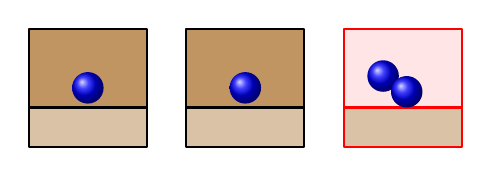
\begin{tikzpicture}[line join=round, line cap=round]
  % Tiroirs en perspective, couleur bois et balles 3D
  \def\drawerwidth{1.5cm}  % Largeur des tiroirs
  \def\drawerheight{1cm}   % Hauteur des tiroirs
  \def\drawerdepth{0.5cm}  % Profondeur (perspective) des tiroirs
  \def\ballradius{0.2cm}   % Taille des balles
  \definecolor{wood}{RGB}{193,154,107} % Couleur bois

  % --- Tiroir 1 ---
  \fill[wood!80!brown] (0,0) -- ++(\drawerwidth,0) -- ++(0,\drawerheight) -- ++(-\drawerwidth,0) -- cycle; % Face avant
  \fill[wood!60!white] (0,0) -- ++(0,-\drawerdepth) -- ++(\drawerwidth,0) -- ++(0,\drawerdepth); % Dessus
  \draw[thick] (0,0) -- ++(\drawerwidth,0) -- ++(0,\drawerheight) -- ++(-\drawerwidth,0) -- cycle;
  \draw[thick] (0,0) -- ++(0,-\drawerdepth) -- ++(\drawerwidth,0) -- ++(0,\drawerdepth);

  % --- Tiroir 2 ---
  \begin{scope}[shift={(2,0)}] % Décalage horizontal
  \fill[wood!80!brown] (0,0) -- ++(\drawerwidth,0) -- ++(0,\drawerheight) -- ++(-\drawerwidth,0) -- cycle;
  \fill[wood!60!white] (0,0) -- ++(0,-\drawerdepth) -- ++(\drawerwidth,0) -- ++(0,\drawerdepth);
  \draw[thick] (0,0) -- ++(\drawerwidth,0) -- ++(0,\drawerheight) -- ++(-\drawerwidth,0) -- cycle;
  \draw[thick] (0,0) -- ++(0,-\drawerdepth) -- ++(\drawerwidth,0) -- ++(0,\drawerdepth);
  \end{scope}

  % --- Tiroir 3 (en évidence) ---
  \begin{scope}[shift={(4,0)}]
  \fill[wood!80!brown, red!10!white] (0,0) -- ++(\drawerwidth,0) -- ++(0,\drawerheight) -- ++(-\drawerwidth,0) -- cycle; % Face avant avec surbrillance
  \fill[wood!60!white] (0,0) -- ++(0,-\drawerdepth) -- ++(\drawerwidth,0) -- ++(0,\drawerdepth); % Dessus
  \draw[thick, red] (0,0) -- ++(\drawerwidth,0) -- ++(0,\drawerheight) -- ++(-\drawerwidth,0) -- cycle;
  \draw[thick, red] (0,0) -- ++(0,-\drawerdepth) -- ++(\drawerwidth,0) -- ++(0,\drawerdepth);
  \end{scope}

  % --- Placement des balles ---
  \shade[ball color=blue] (0.75,0.25) circle (\ballradius); % Tiroir 1
  \shade[ball color=blue] (2.75,0.25) circle (\ballradius); % Tiroir 2
  \shade[ball color=blue] (4.5,0.4) circle (\ballradius);   % Tiroir 3 (deux balles)
  \shade[ball color=blue] (4.8,0.2) circle (\ballradius);
\end{tikzpicture}
\end{center}

% ------------------------------------------------------------
\section{À retenir}\label{sec:retenir}

\begin{retenir}
\begin{itemize}
  \item \emph{Principe des tiroirs} : si l'on place \( n+1 \) objets dans \( n \) tiroirs (\( n \geq 1 \)), au moins un tiroir contient au moins deux objets.
  \item \emph{Forme générale} : si \( k \geq 1 \) et si l'on place \( kn+1 \) objets dans \( n \) tiroirs, au moins un tiroir contient au moins \( k+1 \) objets.
  \item \emph{Méthode} : décider quels sont les objets, choisir les tiroirs (la partie difficile : mois, restes d'une division, petites figures\ldots), puis comparer leurs nombres.
\end{itemize}
\end{retenir}

% ------------------------------------------------------------
\section{Exercices}\label{sec:exercices}

\subsection*{Quelques exercices simples}

\exochap{recueil-3-01-meme-sexe}{Deux personnes du même sexe}

\exochap{recueil-3-02-anniversaires}{Anniversaires}

\exochap{recueil-3-03-cheveux}{Cheveux sur la tête}

\exochap{recueil-3-04-anniversaires-multiples}{Anniversaires multiples}

\exochap{recueil-3-05-perles-boites}{Perles dans des boîtes}

\exochap{recueil-3-06-ligne-triangle}{Ligne dans un triangle}

\exochap{recueil-3-07-tetraedre}{Intersection d'un tétraèdre}

\exochap{recueil-3-08-cible-triangulaire}{Trous sur une cible triangulaire}

\exochap{recueil-3-09-periode-fraction}{Période d'une fraction}

\exochap{recueil-3-10-decimaux-infinis}{Décimaux infinis}

\exochap{recueil-3-11-deux-chiffres}{Nombres à deux chiffres}

\exochap{recueil-3-12-divisibilite-coprime}{Divisibilité et nombres premiers entre eux}

\subsection*{Quelques exercices}

\exochap{recueil-3-13-divise-un-autre}{Un nombre en divise un autre}

\exochap{recueil-3-14-bezout-naturels}{Une relation de Bézout}

\exochap{recueil-3-15-differences-egales}{Quatre différences égales}

\exochap{recueil-3-16-neuf-points}{Neuf points à coordonnées entières}

\exochap{recueil-3-17-repunits}{Un multiple fait de 1}

\exochap{recueil-3-18-produit-differences}{Produit de différences}

% ------------------------------------------------------------
\section{Problèmes}\label{sec:problemes}

\subsection*{Quelques problèmes simples}

% Note d'origine : Problème E7
\probleme{recueil-3-p1-cinq-points-grille}{Cinq points dans une grille}

\probleme{recueil-3-p2-connaissances}{Des gens dans une pièce}

\probleme{recueil-3-p3-tournoi-echecs}{Tournoi d'échecs}

\probleme{recueil-3-p4-erdos-szekeres}{Erdős et Szekeres}

\subsection*{Quelques problèmes}

\probleme{recueil-3-p5-puissance-terminaison}{Une puissance bien terminée}

\probleme{recueil-3-p6-ramsey-six}{Six personnes}

\probleme{recueil-3-p7-scientifiques}{Les dix-sept scientifiques}

\probleme{recueil-3-p8-sous-ensembles}{Deux sous-ensembles de même somme}

\probleme{recueil-3-p9-couronne}{Points dans une couronne}

\probleme{recueil-3-p10-cercles-carre}{Cercles dans un carré}

\probleme{recueil-3-p11-sept-points}{Sept points dans un disque}

\probleme{recueil-3-p12-differences}{Différences imposées}

\end{document}
